\section{Metodología}
\subsection{Medición de dimensiones del recinto}
\noindent Para caracterizar el recinto, es necesario tener las dimensiones de cada sala. Parte del detalle de las dimensiones fueron proporcionadas por el encargado del Campus Los Canelos. En la figura \ref{fig: planos CAD} se puede observar una vista superior de las salas a estudiar.

\begin{figure}[H]
    \centering
    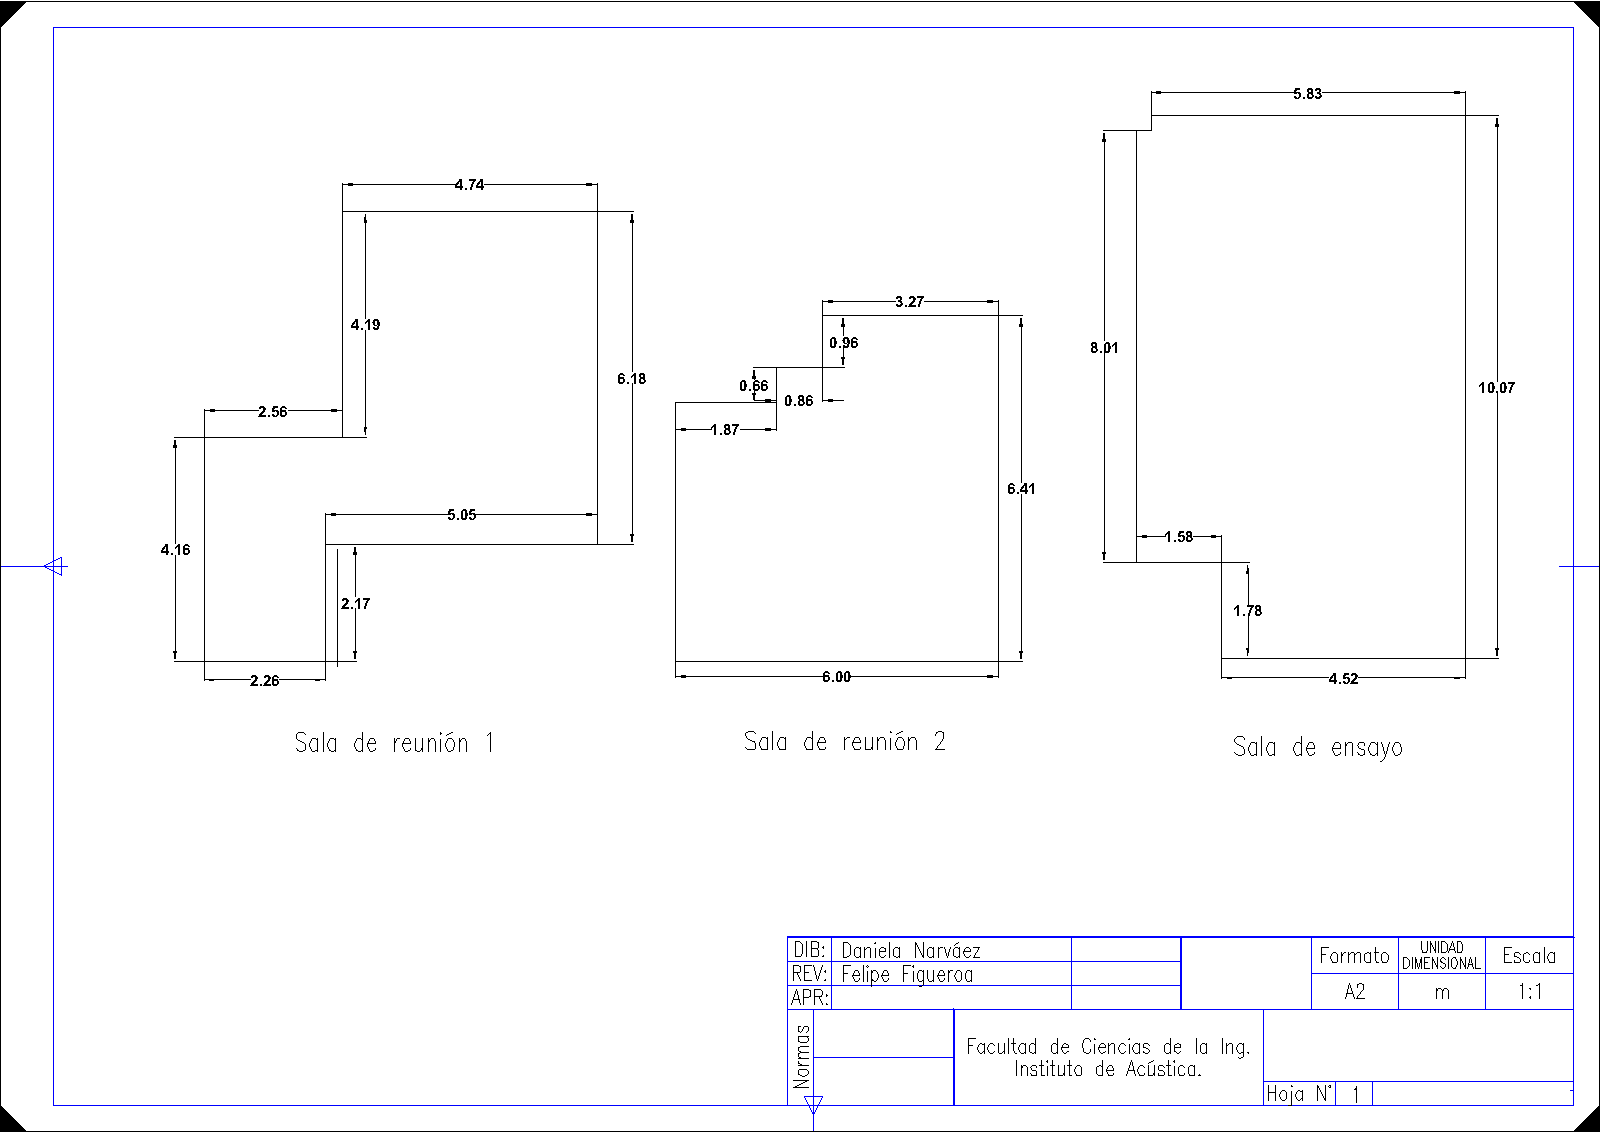
\includegraphics[scale=0.3]{Imagenes/Planos/Planos.png}
    \caption{Planos de salas de reuniones y sala de ensayo Campus los canelos}
    \label{fig: planos CAD}
\end{figure}
%insertar imágenes


\subsection{Medición de parámetros acústicos del recinto}
\noindent Para poder caracterizar acústicamente los salones, se necesita medir parámetros como el ruido de fondo y tiempo de reverberación de cada sala. Para esto se utilizará los siguientes instrumentos:

\begin{table}[H]
    \centering
    \caption{Instrumentación utilizada para las mediciones}
    \label{tab:instrumentacion}
    \resizebox{\textwidth}{!}{%
    \begin{tabular}{|l|l|}
    \hline
    \textbf{Instrumentos} & \textbf{Uso}\\ \hline
    Sonómetro Cirrus CR:$171$B & Medir nivel de presión sonora equivalente \\ \hline
    Micrófono Behringer ECM$8000$ & Recibir el nivel de las fuentes\\\hline
    Conectores XLR & Enviar señal de audio\\ \hline
    Interfaz de audio TASCAM US $4$x$4$ & Procesar señales de audio\\ \hline
    Cinta métrica & Medir distancia de fuente y micrófonos \\ \hline
    Termómetro e higrómetro digital & Medir temperatura y humedad en el lugar de medición\\ \hline
    Protectores auditivos & Proteger oídos de la exposición de sonidos fuertes  \\ \hline
    Notebook con software ARTA & Procesar y analizar señales   \\ \hline
    Globos & Fuente impulsiva \\ \hline
    
    \end{tabular}
    }
\end{table}

\subsubsection{Ruido de fondo}
\noindent Para medir el ruido de fondo se utilizó el sonómetro Cirrus midiendo 5 minutos hasta que el nivel de presión sonora equivalente se estabilice, basándose en el procedimiento descrito en el D.S. $38/11$ \cite{ds:ds38}.
\begin{figure}[H]
    \centering
    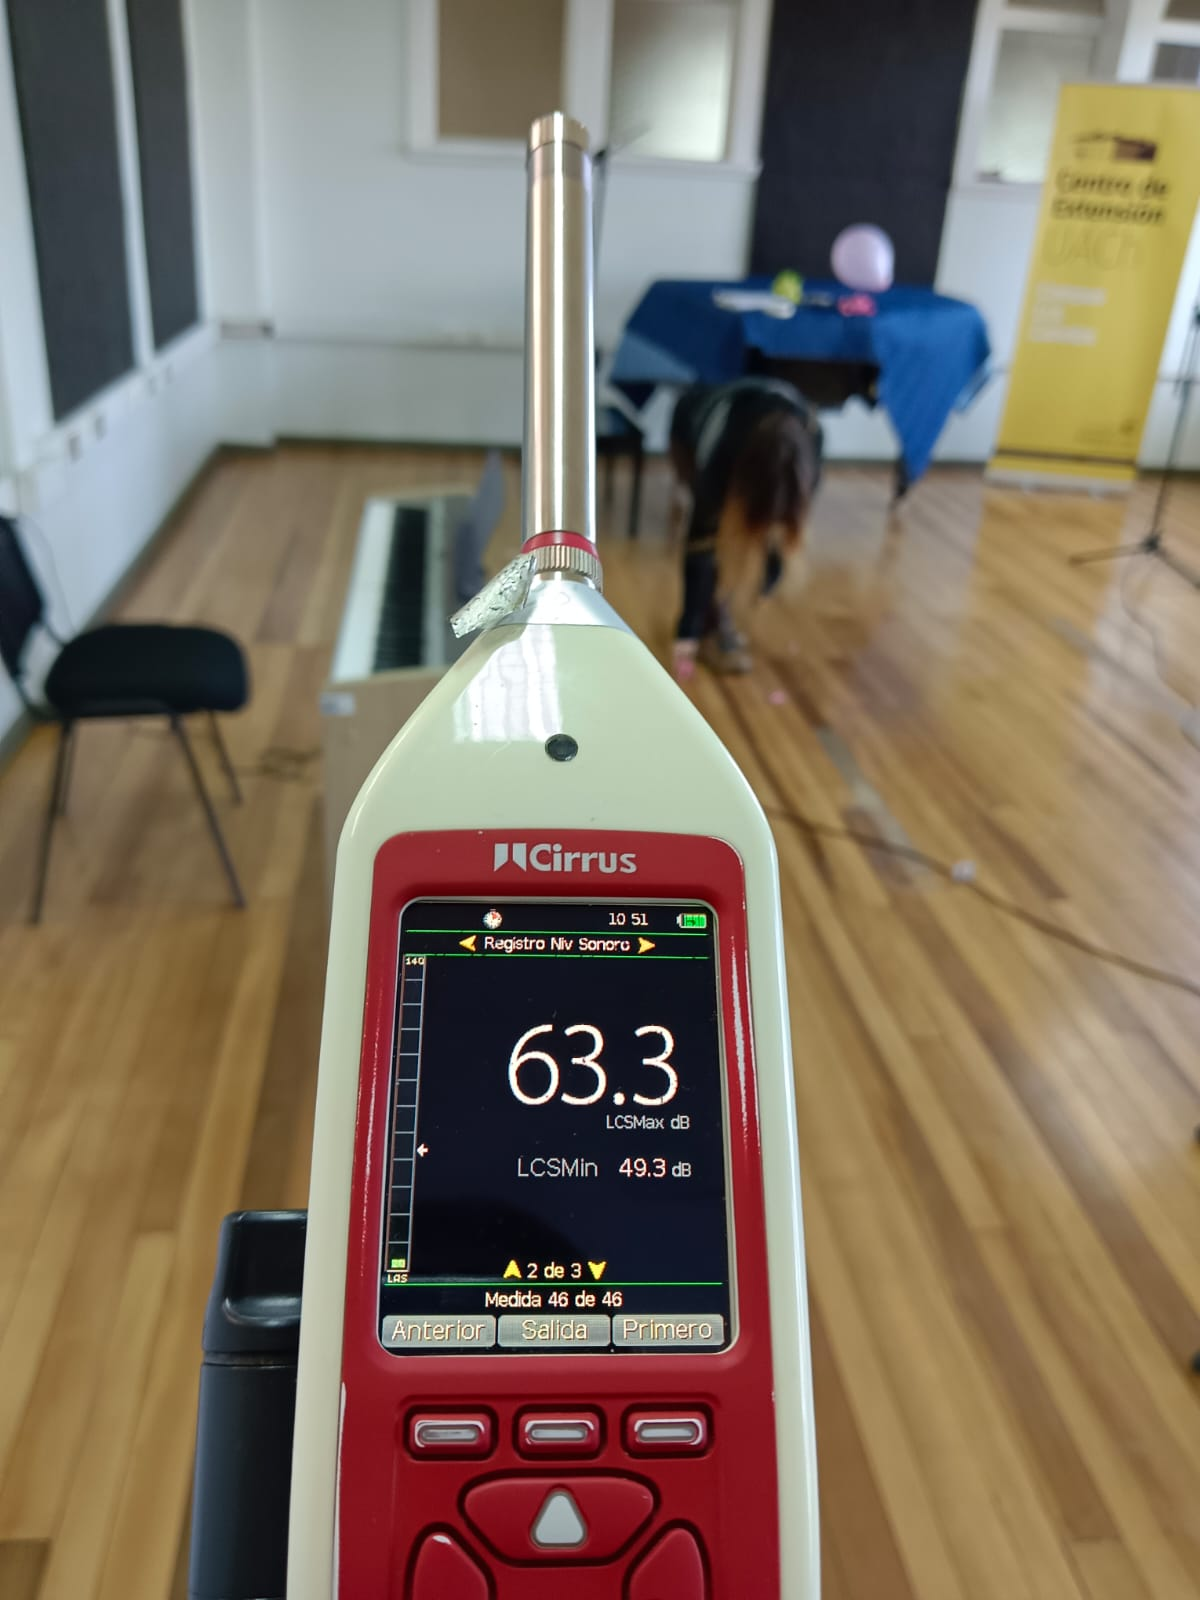
\includegraphics[scale=0.15]{Imagenes/mediciones/medicionRDF.jpeg}
    \caption{Medición de ruido de fondo}
    \label{fig: medicionRDF}
\end{figure}
\subsubsection{Tiempo de reverberación}
\noindent Para la medición de tiempo de reverberación se siguió el procedimiento que indica la norma ISO $3382$-$2$ \cite{ISO3382-2}, utilizando el método de respuesta impulso en cada una de las salas, utilizando globos como fuente impulsiva.
En cada sala de reuniones se realizan dos posiciones de fuente y tres de micrófono, y para la sala de ensayo se utilizan dos posiciones de fuente y cuatro de micrófono, realizando dos mediciones para cada combinación de fuente-micrófono. En el anexo \ref{subsec: posiciones RT} se encuentran los planos con las posiciones de fuente y micrófono utilizadas en cada salón.

\begin{figure}[H]
    \centering
    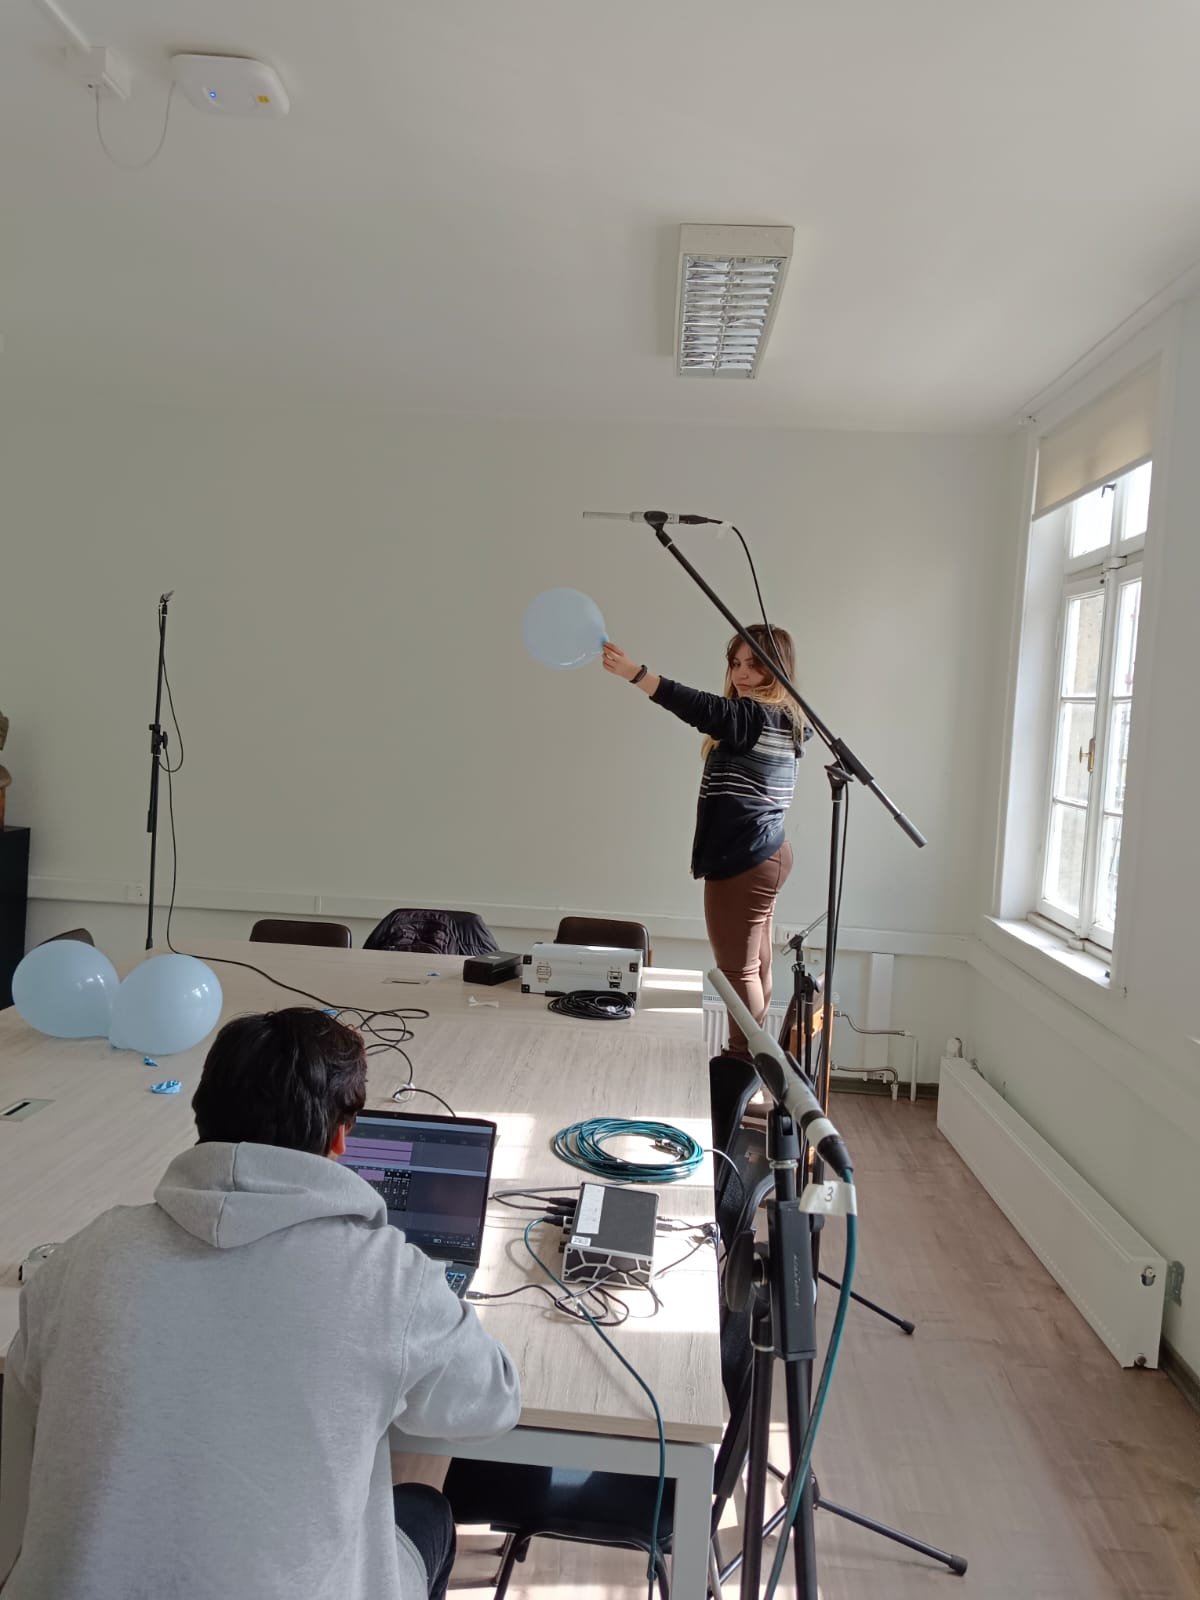
\includegraphics[scale=0.15]{Imagenes/mediciones/medicionRT.jpeg}
    \caption{Medición de ruido de tiempo de reverberación}
    \label{fig: medicionRT}
\end{figure}



